\documentclass[../../main.tex]{subfiles}

\graphicspath{{../../fig/}}
\setcounter{section}{0}

\begin{document}
\chapter{Simons Observatory実験}
\section{Simons Observatory実験}
Simons Observatory実験(以後、SOと呼ぶ)は、チリのアタカマ砂漠を拠点とする史上最大規模の地上CMB観測実験である。
現在、口径$0.5\ \mathrm{m}$の小口径望遠鏡(Small Aperture Telescope, SAT)3台と、
口径 $6\ \mathrm{m}$の大口径望遠鏡(Large Aperture Telescope, LAT)1台を用いた観測が進められており\cite{so:current_status}、
今後さらに日本製の1台のSAT(JSAT)と、イギリス製の2台のSATが追加される予定である。図\ref{fig:so_site}に観測サイトの概観を示す。
検出器としてはTES(Transition Edge Sensor)ボロメータを採用しており、SATにはそれぞれ約1万個ずつ、LATには約3万個の検出器が搭載されている。
多数の検出器を用いたCMB偏光の高精度測定は、さまざまな物理へのアプローチを可能にする。
例えば、SATではインフレーションに由来する原始重力波の検出をテンソルスカラー比$r$にして$\sigma(r)=0.003$の精度で行う。
また、LATではニュートリノの有効世代数$N_\mathrm{eff}$を$\sigma(N_{\mathrm{eff}})=0.07$、ニュートリノ質量和$\Sigma m_\nu$を$\sigma(\Sigma m_\nu)=\SI{0.04}{eV}$の精度での測定を目指す\cite{so:science_forecast}。
\begin{figure}[H]
    \centering
    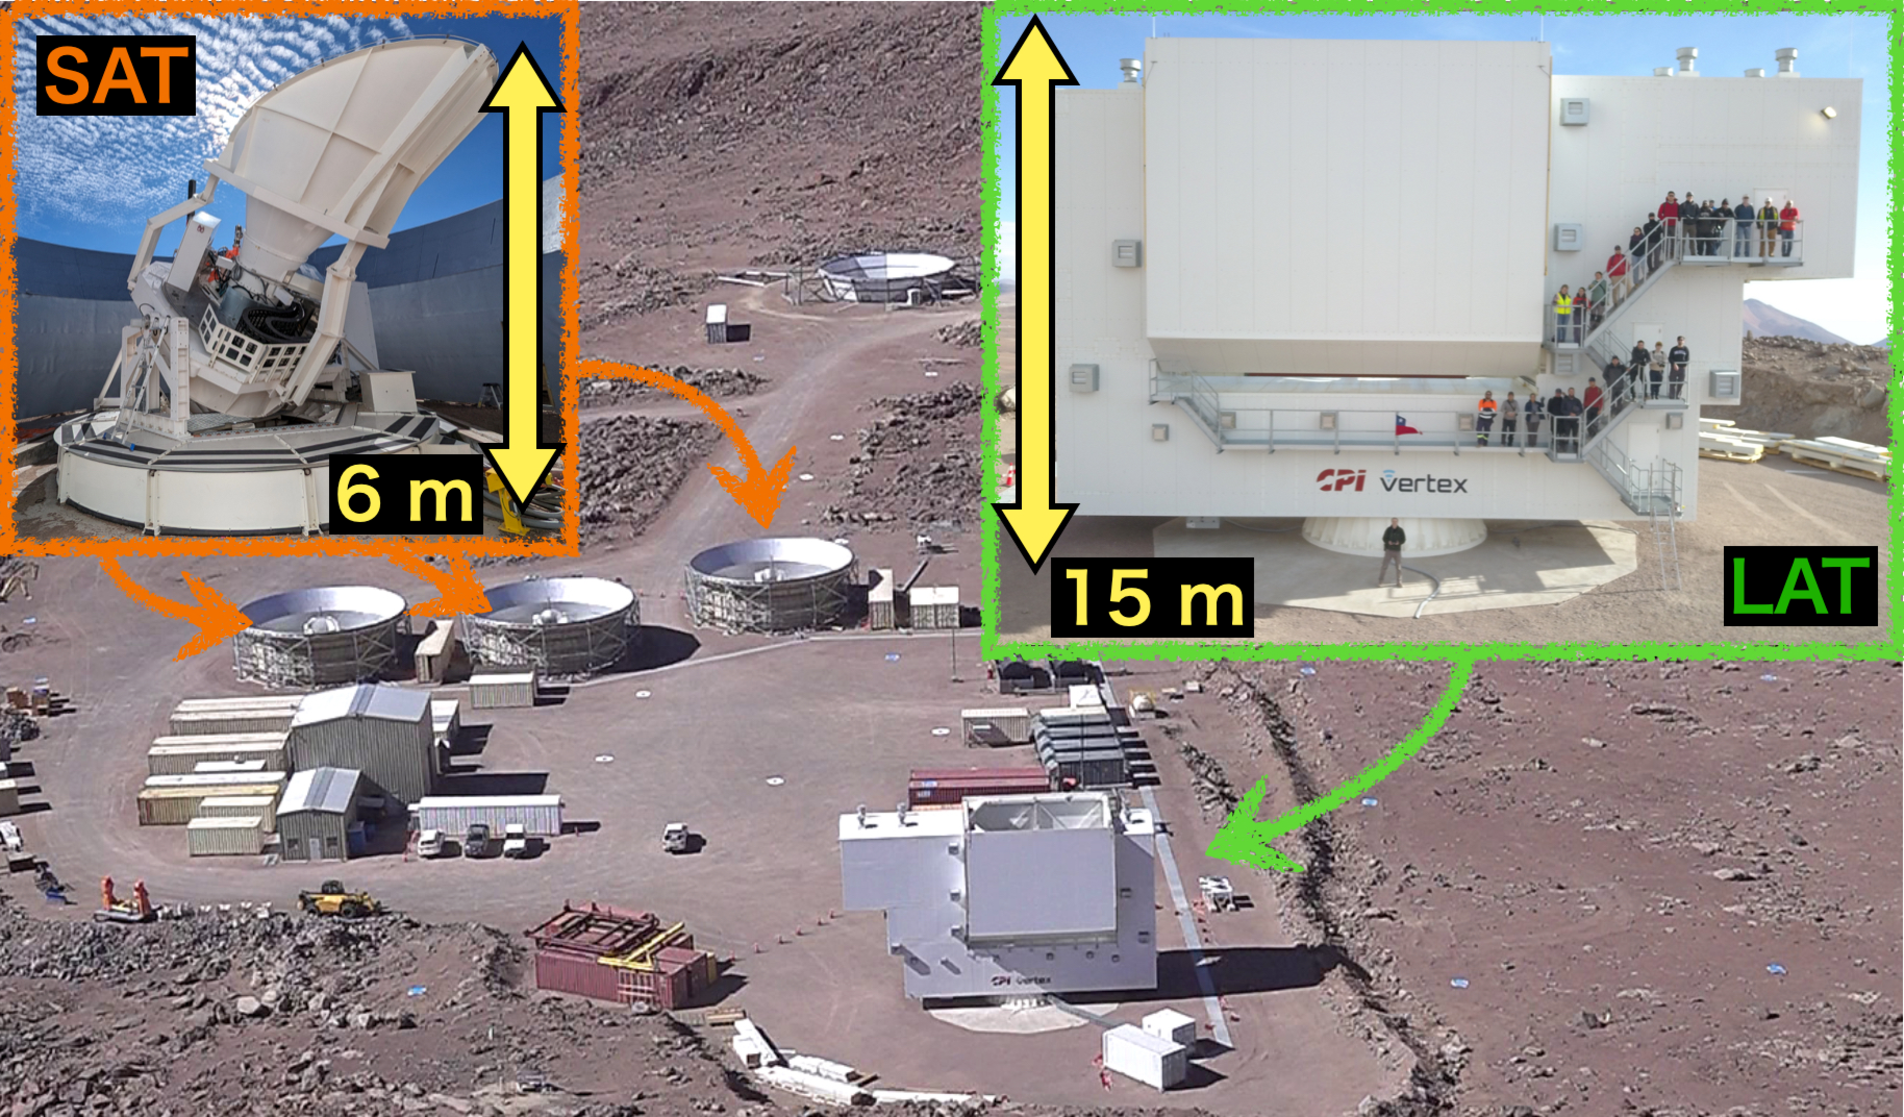
\includegraphics[width=1.0\textwidth]{simons_observatory/so_site.pdf}
    \caption{Simons Observatory実験の観測サイトの概観。
    左側に3台並んで建設されているのがSATであり、右側手前に1台建設されているのがLATである。}
    \label{fig:so_site}
\end{figure}

立体角 $\Omega$ 、開口面積 $A$、観測波長 $\lambda$ について、回折限界の関係式\cite{text_radioastro}
\begin{equation}
    \Omega \approx \dfrac{\lambda^2}{A}
\end{equation}
を考えると、より大きな口径$A$を持つ望遠鏡ほどより高い角度分解能を有し、小角度の相関を観測するのに適していることがわかる。
その一方で、大口径の望遠鏡は一度に観測できる範囲も小さくなるため、大角度の相関を観測するのに時間を要し、時間変動による大気揺らぎの影響を受けやすくなってしまう。
以上の理由から、小口径で大角度相関を調べるSATと、大口径で小角度相関を調べるLATを組み合わせることで、
広大な$\ell$に渡ってCMBパワースペクトルの精密な測定を行い、前述した様々な物理へのアプローチを実現する。
\section{Small Aperture Telescope (SAT)}
前述の通り、SATは小口径の望遠鏡であり、CMBの大角度相関、特に$30<\ell<300$を観測するために最適化されている。
3台のSATのうち2台は$\SI{93}{GHz}$、$\SI{145}{GHz}$帯(MF帯)での観測を行い、1台は$\SI{225}{GHz}$、$\SI{280}{GHz}$帯(UHF帯)での観測を行う。
また、日本グループが主導して追加される1台のSATは$\SI{27}{GHz}$、$\SI{39}{GHz}$帯(LF帯)での観測を行う。
このように複数の帯域に渡って観測を行う理由は、星間物質中の塵が熱的に放射するダスト放射や、
超新星残骸中の磁場などによって加速された荷電粒子が放出するシンクロトロン放射などのフォアグラウンドを除去するためである。
図\ref{fig:so_noise_freq}にSATの観測帯域と、CMB偏光信号、ダスト放射、シンクロトロン放射の輝度温度の周波数依存性を示す。
\begin{figure}[H]
    \centering
    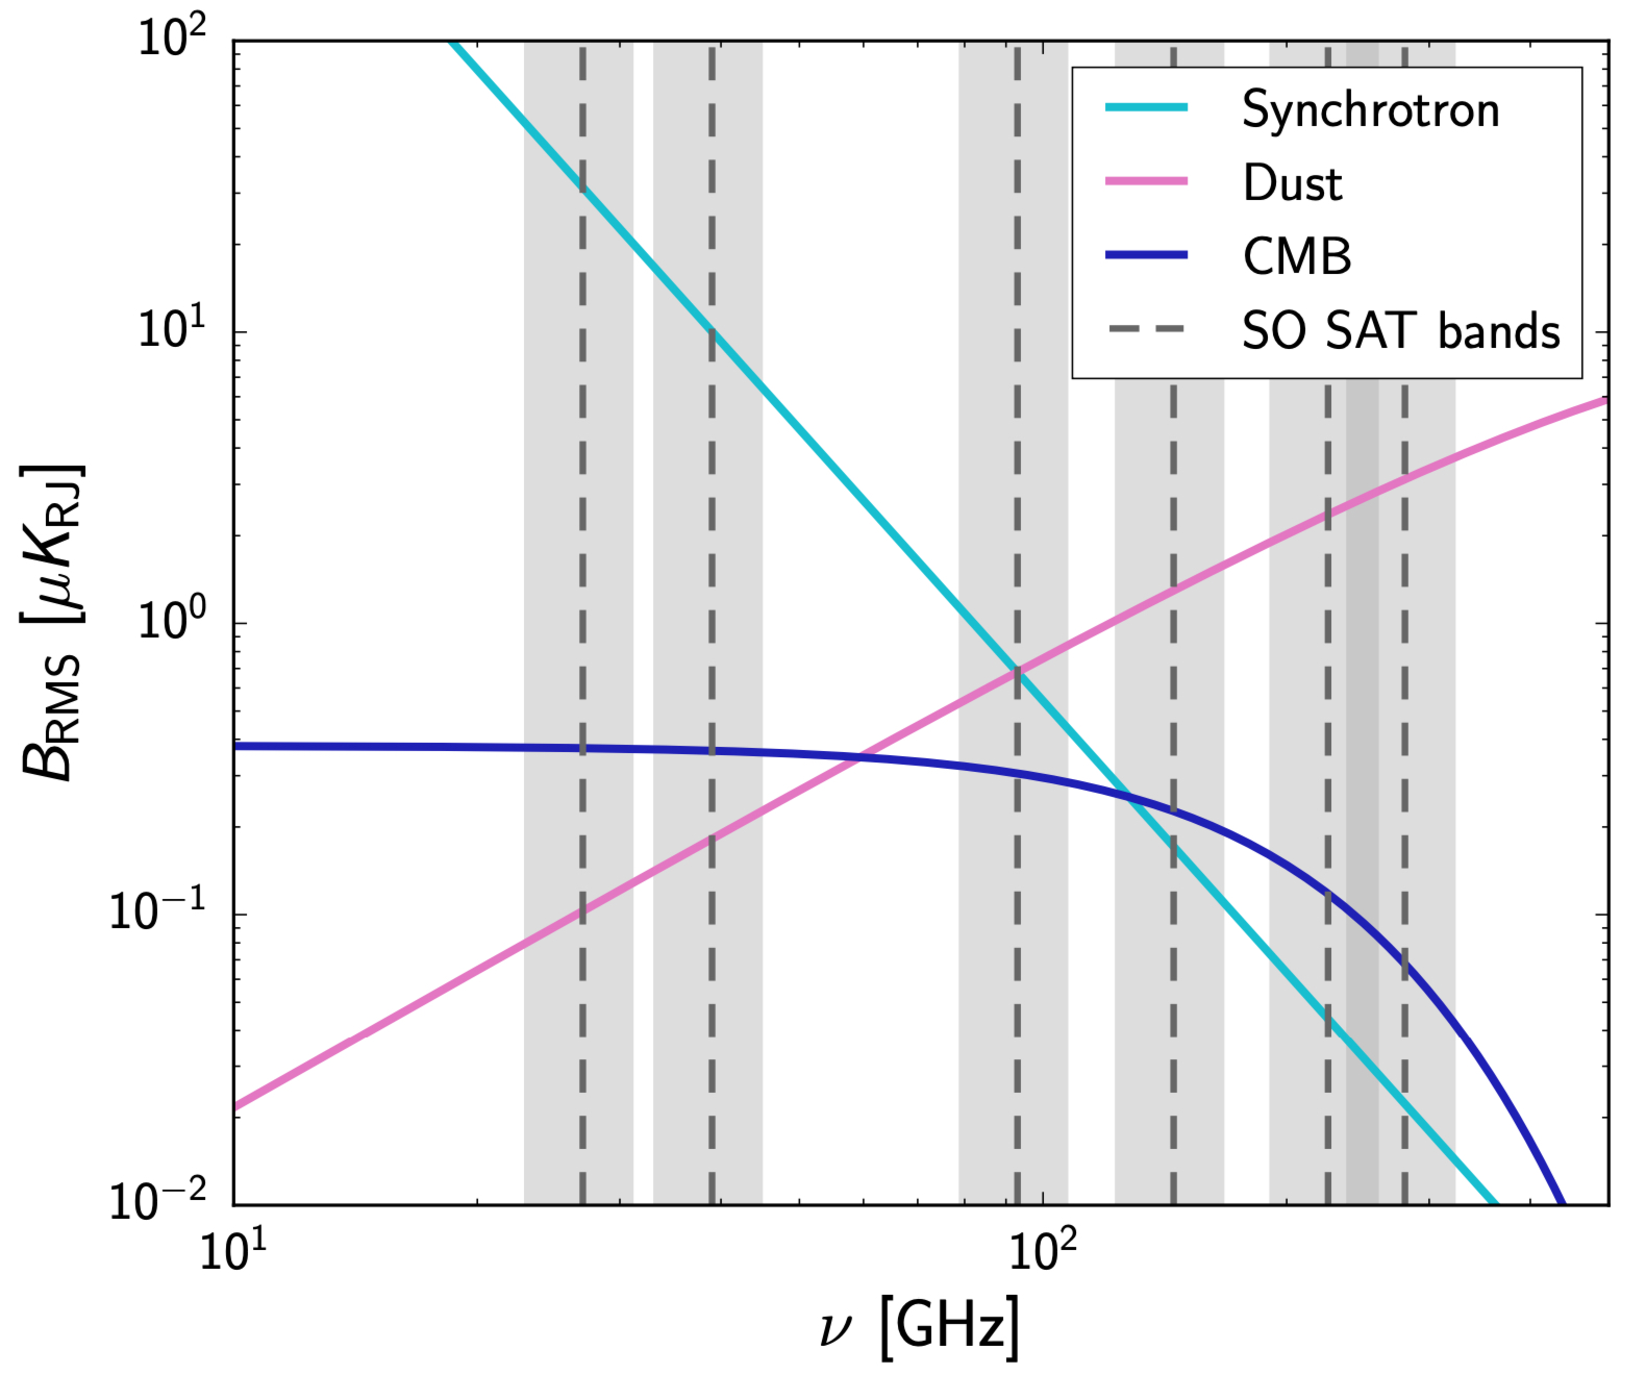
\includegraphics[width=0.75\textwidth]{simons_observatory/so_noise_freq.pdf}
    \caption{SATの観測帯域と、CMB偏光信号、ダスト放射、シンクロトロン放射の輝度温度の周波数依存性の比較。}
    \label{fig:so_noise_freq}
\end{figure}

図\ref{fig:so-sat_baffle}にSATの概観を示す。
SATにはフォアバッフル・コムービングシールド・グラウンドスクリーンの3つのバッフル群を用いて地面からの熱放射や、
近くの山からの照り返しを受信機が受信してしまうことで生じるノイズを抑えている\cite{Kiuchi_2020}。
フォアバッフルはSATの受信機に取り付けられており、コムービングシールドはSATを支える構造物に取り付けられ、望遠鏡と共に動く。
グラウンドスクリーンはSATを取り囲むように設置され、地面からの照り返しを遮断する。

図\ref{fig:so-sat_angle}にSATの回転軸を示す。
SATはelevationと呼ばれる仰角方向の角度と、azimuthと呼ばれる方位各方向に回転させることができる。
また、一部のSATではboresightと呼ばれる視線方向に対する回転も可能である。
\begin{figure}[H]
    \centering
    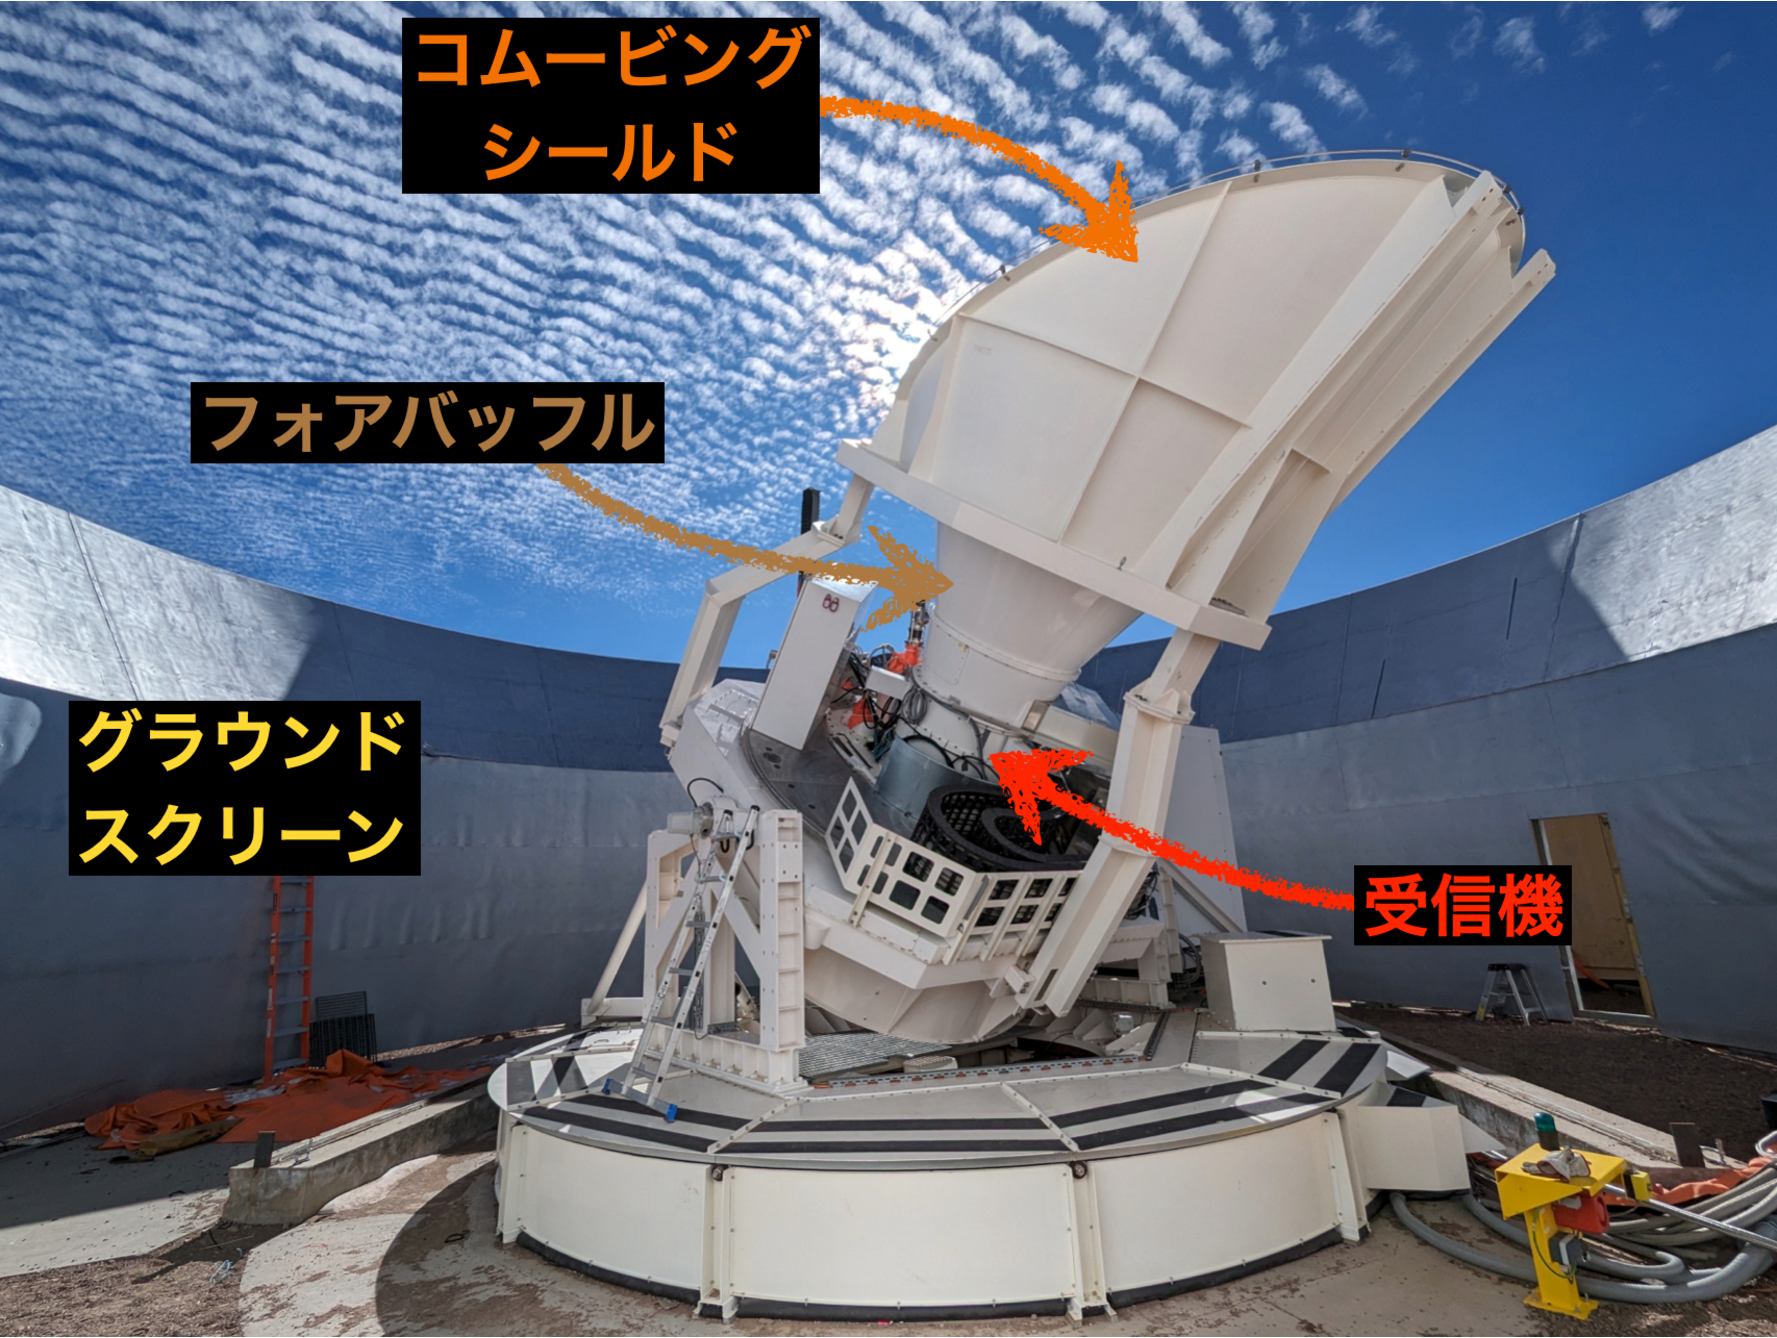
\includegraphics[width=0.75\textwidth]{simons_observatory/sat_baffle.pdf}
    \caption{SATのもつ3つのバッフル群。これらのバッフルによって、地面からの熱放射や近隣の山からの照り返しに由来するノイズを削減する。}
    \label{fig:so-sat_baffle}
\end{figure}
\begin{figure}[H]
    \centering
    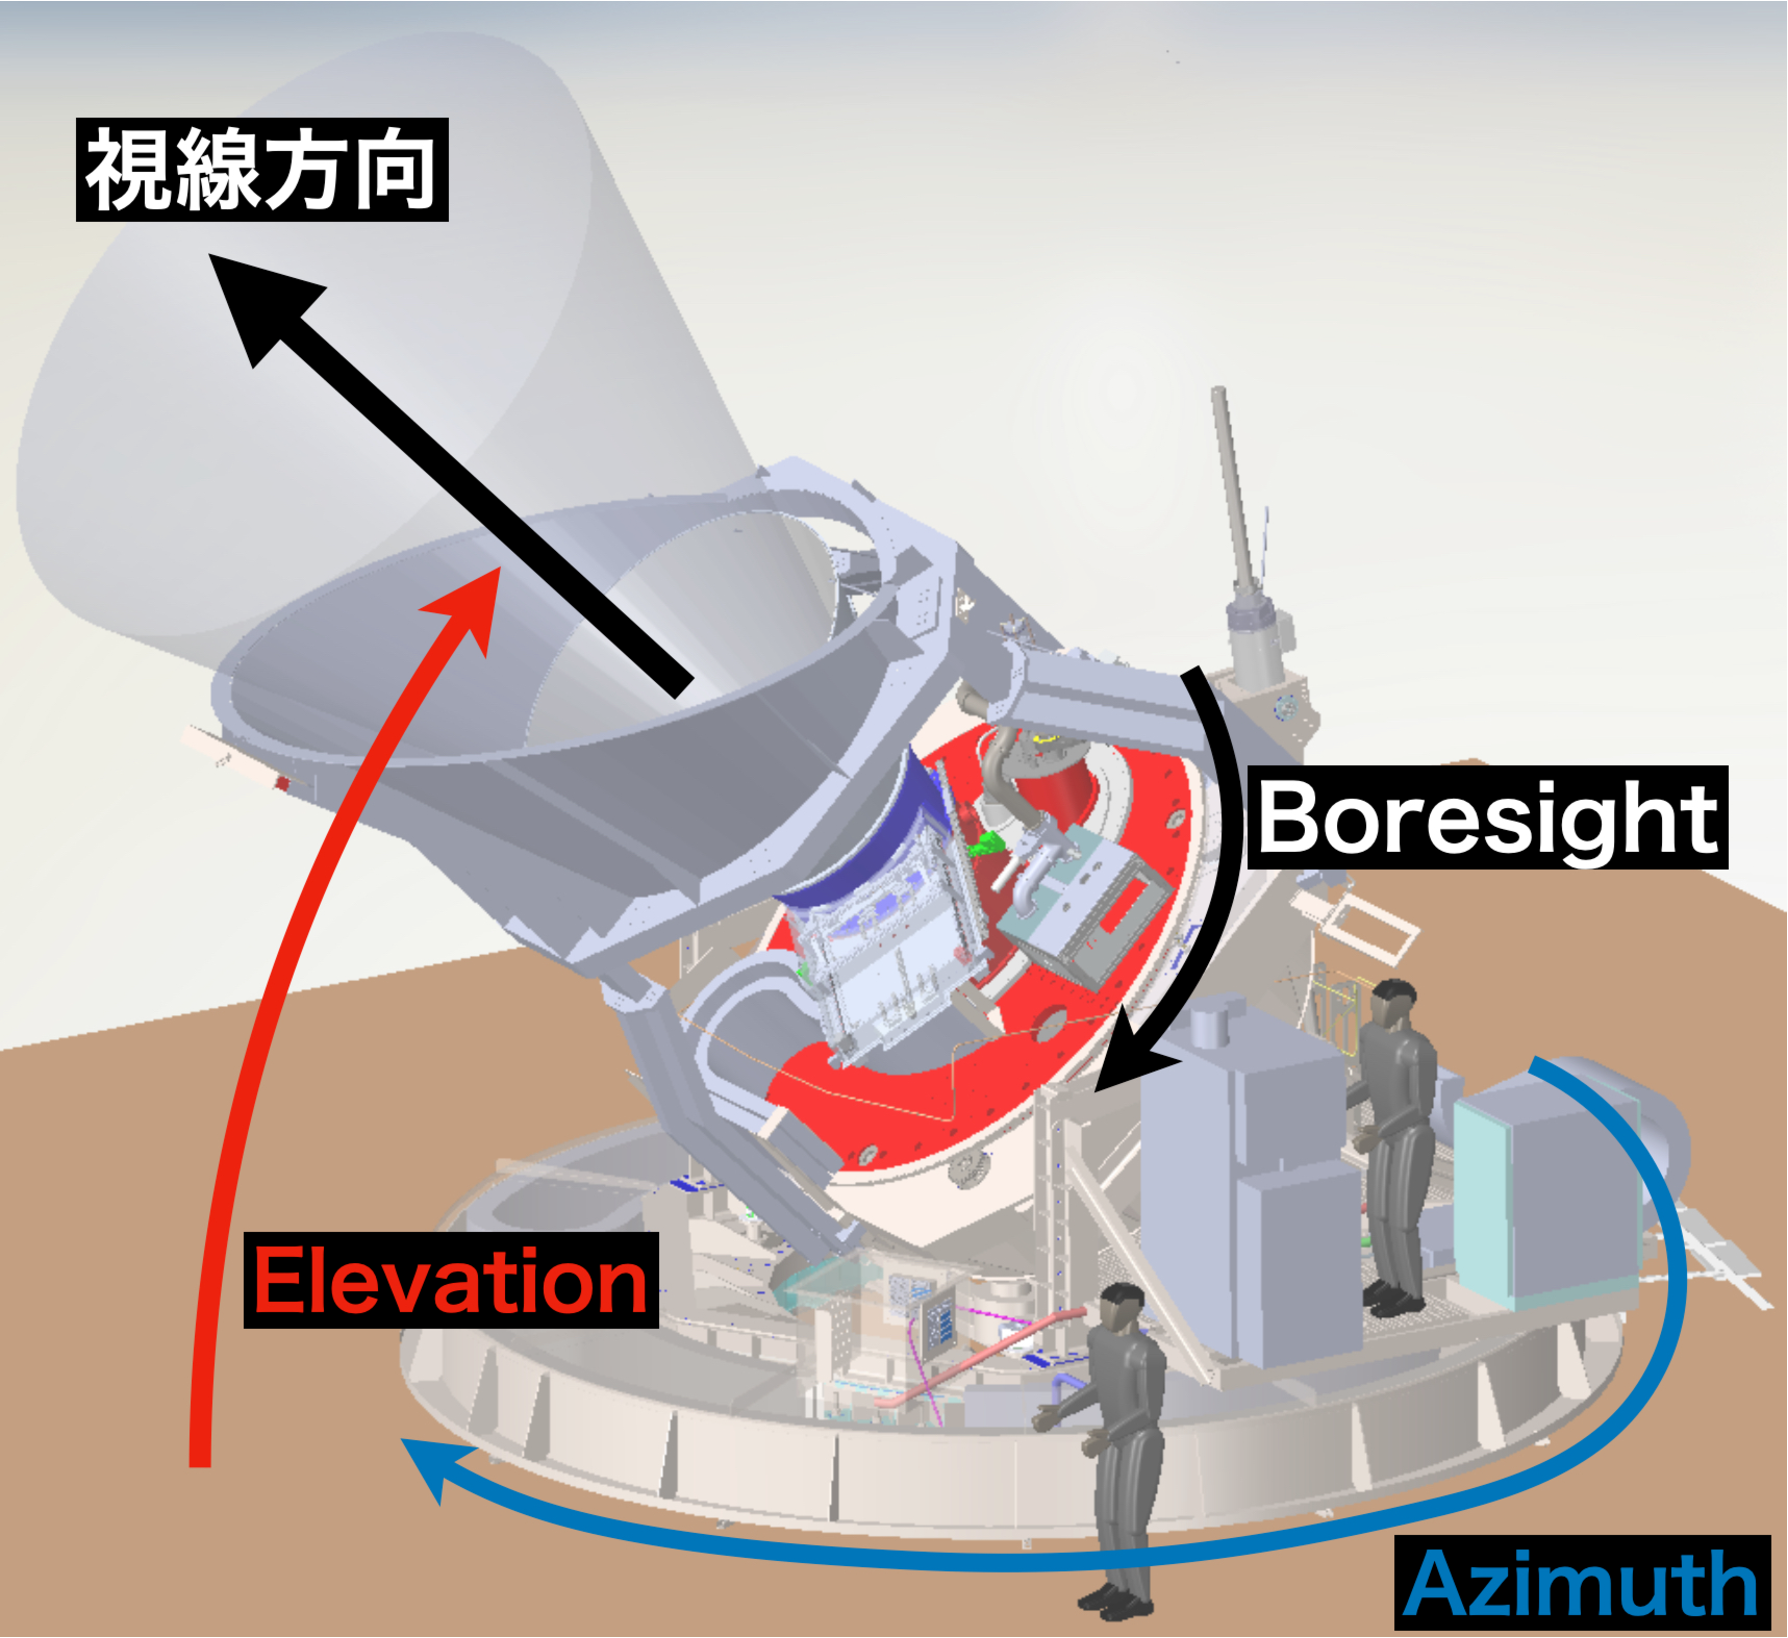
\includegraphics[width=0.65\textwidth]{simons_observatory/sat_angle.pdf}
    \caption{SATの回転軸。$\mathrm{Elevation}=50\tcdegree$がSATの基本姿勢である。}
    \label{fig:so-sat_angle}
\end{figure}

図\ref{fig:so-sat}にSATの受信機部分の断面図を示す。
空から降ってきた光は窓を透過後、後述する極低温連続回転式半波長板(HWP)を通過・変調されたのちに光学筒を通って焦点面検出器に到達する。
光学筒には3枚のシリコンレンズが搭載されており、入射してきた光を集光する。
焦点面には後述するTESボロメータと呼ばれる超伝導検出器が搭載されており、受信機に斜めに挿さっている希釈冷凍機システムによって$\SI{100}{mK}$にまで冷却されている\cite{galitzki2024simonsobservatorydesignintegration}。

望遠鏡の窓の前面には、本論文にて扱うスパースワイヤーグリッドを用いた偏光角較正装置が取り付けられている。
光学系の目の前に設置されているため、望遠鏡の窓から焦点面に至るまでのすべての光学系により生まれる偏光角の系統誤差を丸ごと較正することができる。
また、望遠鏡の視野を覆うように配置されているため、すべての検出器を一度に較正することができる。
\begin{figure}[H]
    \centering
    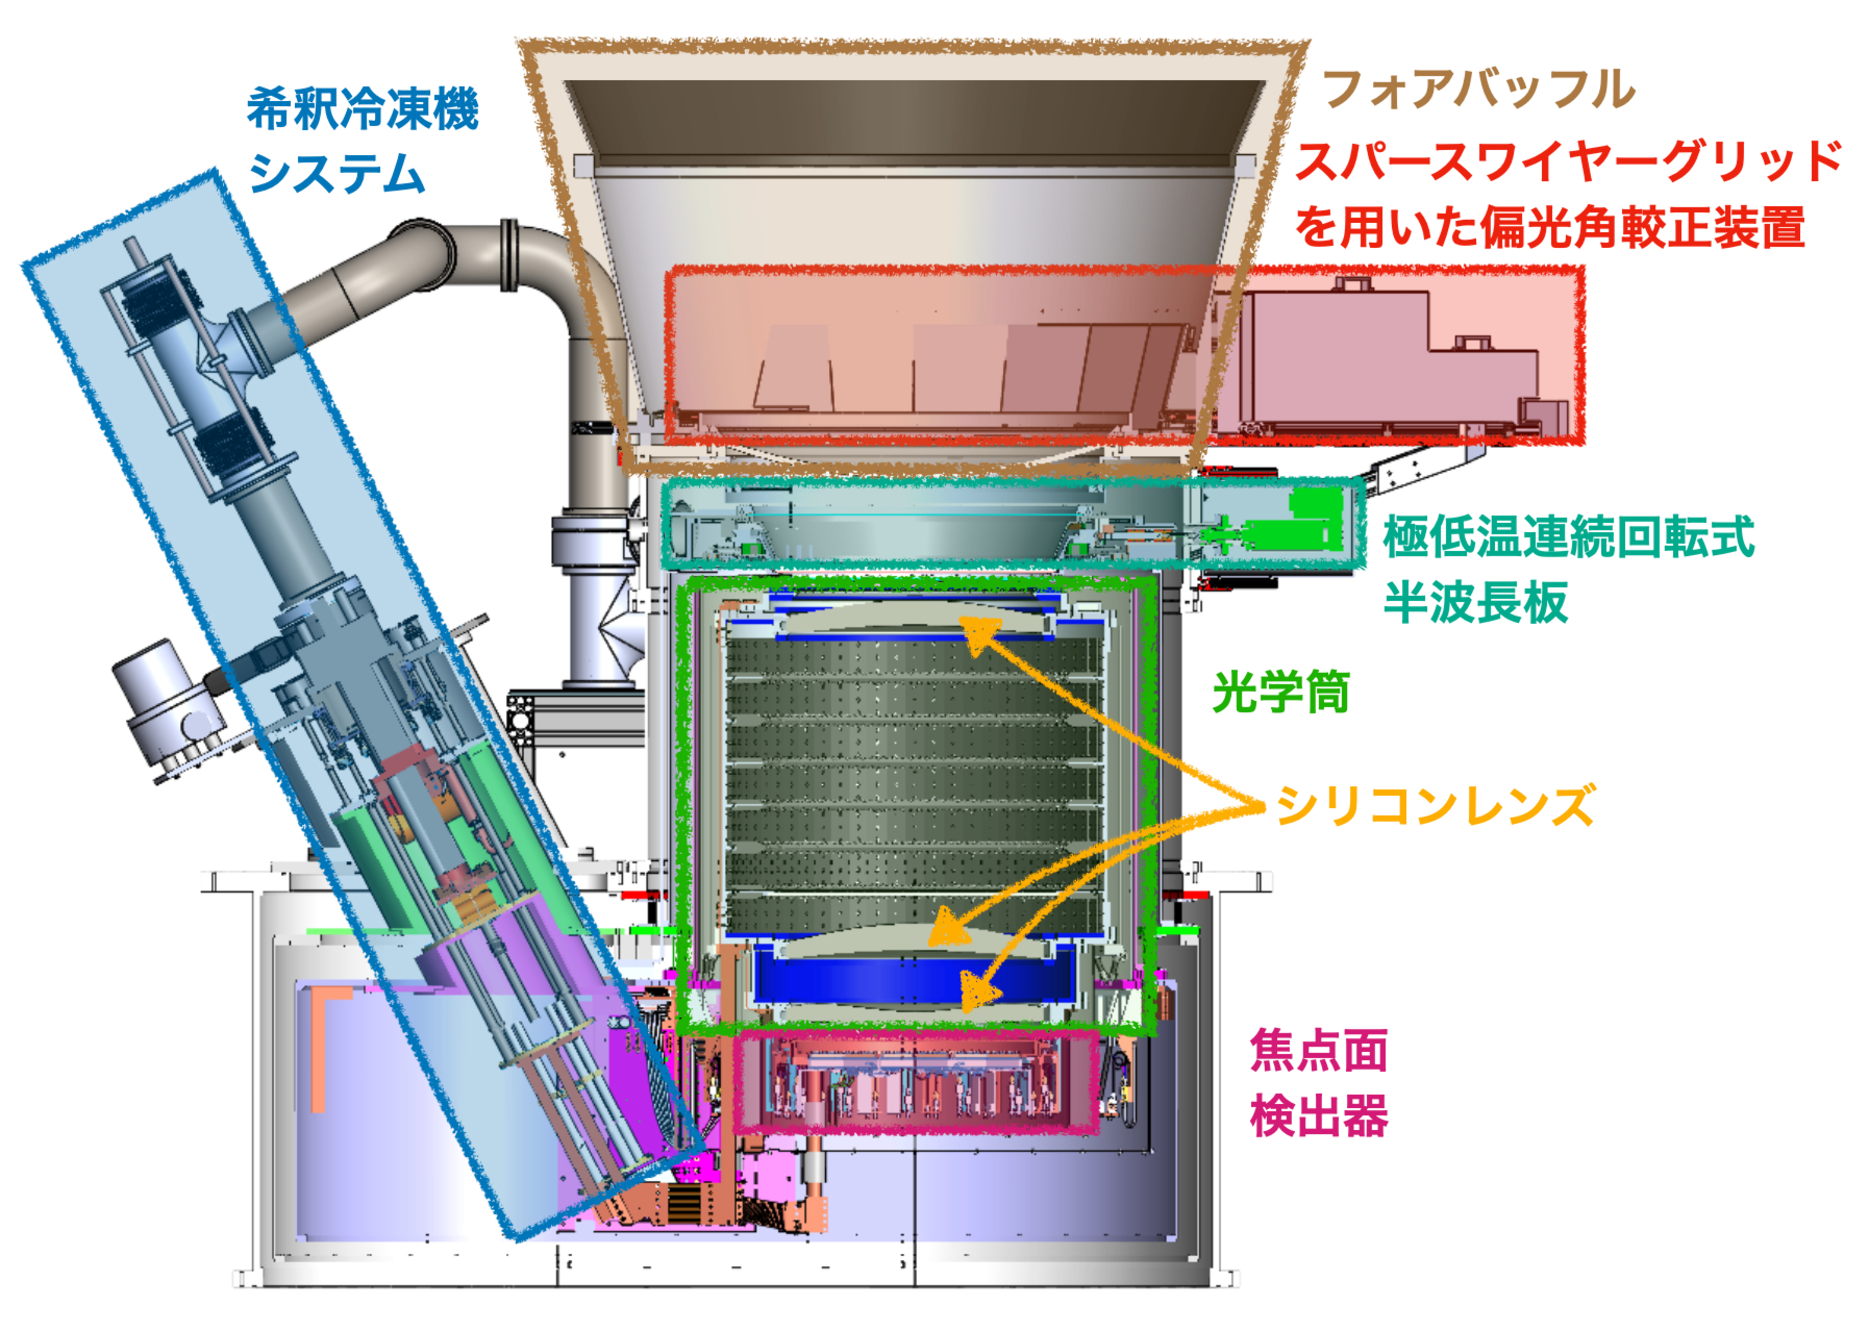
\includegraphics[width=1.0\textwidth]{simons_observatory/sat_danmen.pdf}
    \caption{SATの受信機部分の断面図}
    \label{fig:so-sat}
\end{figure}

\subsection{焦点面検出器}
超伝導物質は転移点付近で電気抵抗が急激にゼロに近づく性質を持つ。
転移点近傍の温度に制御された超伝導物質に吸収体を接続すると、光が入射してきた場合に吸収体が光を熱に変換し、超伝導物質を温める。
これによりその温度が転移点を超え、超伝導物質の電気抵抗が急激に増加する。
この電気抵抗が急激に増加するのを読み取ることで、入射した光の強度を測定する装置、すなわちボロメータを作ることができる。
このような装置はTES(Transition Edge Sensor)ボロメータと呼ばれる。

SOの焦点面検出器には、TESボロメータが使用されている。
TESボロメータにはOMT(Ortho-Mode Transducer)とフィードホーンが取り付けられており、
入射してきた光をフィードホーンによってOMTに導き、OMTによって直交する2つの偏光方向に分ける\cite{duff2024simonsobservatoryproductionlevelfabrication}。
分けられた光はそれぞれ別のTESボロメータに導かれ、各TESボロメータで光の強度が測定される。
このようにして、焦点面検出器は入射してきた光の偏光方向に対して感度を獲得している。

\subsection{極低温連続回転式半波長板 (HWP)}
\label{sec:HWP}
宇宙から降り注ぐCMBと望遠鏡の間には地球の大気がある。
そして大気の無偏光熱放射は時事刻々と変化する(つまり、常に揺らいでいる)。
これは大気による $1/f$ ノイズとして知られ、CMB偏光観測実験においては、このノイズとCMB偏光信号を分離することが重要である。
SATでは、この大気による熱放射を取り除くために、極低温連続回転式半波長板(cryogenic continuously rotating Half-Wave Plate, 以後、単にHWPと呼ぶ)を用いる\cite{so:hwp_yamada}。

一般に、HWPは複屈折の特性を持つ素材からなり、素子中のある決まった軸(光軸)に対して電場成分を反転させる。
すなわち、HWPに入射する光の電場 $\bm{E}$ はHWPを通過することで
\begin{align}
    E_{1} &= E_{1} \\
    E_{2} &= -E_{2}
\end{align}
となる。ここで、1軸はHWPの光軸、2軸は1軸に垂直なHWP平面上の軸を表し、1軸に対して電場成分が反転している。
入射光として偏光角がHWPの1軸から測って$\chi$であるような直線偏光した光を考える。
HWPを通過した後の偏光角は$-\chi$となり、偏光が1軸対称に反転、つまり$-2\chi$だけ変化する(図\ref{fig:so-hwp_satoru})。
この性質により、ストークスパラメータ(定義は\ref{chap:stokes}を参照)が
それぞれ$I_{\mathrm{in}}(t), Q_{\mathrm{in}}(t), U_{\mathrm{in}}(t)$であるような直線偏光した入射光を、
HWPを通過したあとに1軸方向に感度を持つ片偏波のアンテナで電場強度を測った際の出力信号$d_m(t)$は
\begin{equation}
    d_{\mathrm{m}}(t) = I_{\mathrm{in}}(t) + \varepsilon\Re\qty[\qty(Q_{\mathrm{in}}(t)+iU_{\mathrm{in}}(t))\exp(-i 4\chi)]
\end{equation}
となる。ここで、$\varepsilon$ は変調効率である。つまり、SOのように、HWPを$\SI{2}{Hz}$で回転させると、連続的に入射する直線偏光の信号を$\SI{8}{Hz}$に変調して出力することになる。
HWPの角振動数を$\omega_{\mathrm{HWP}}$とし、初期位相を$\chi_0$とすると、$\chi(t) = \omega_{\mathrm{HWP}}t + \chi_{0}$と表され、出力信号は
\begin{equation}
    d_{\mathrm{m}}(t) = I_{\mathrm{in}}(t) + \varepsilon\Re\qty[\qty(Q_{\mathrm{in}}(t)+iU_{\mathrm{in}}(t))\exp(-i \qty(4\omega_{\mathrm{HWP}}t + 4\chi_0))]
\end{equation}
となる。検出器はある偏光角方向$\theta_{\mathrm{det}}$にのみ感度を持つため、最終的に検出器が読み出す信号$d_{\mathrm{m}, \mathrm{det}}$は
\begin{equation}
    \label{eq:so-hwp_modulation}
    d_{\mathrm{m}, \mathrm{det}}(t) = I_{\mathrm{in}}(t) + \varepsilon\Re\qty[\qty(Q_{\mathrm{in}}(t)+iU_{\mathrm{in}}(t))\exp\qty{-i \qty(4\omega_{\mathrm{HWP}}t + 4\chi_0 - 2\theta_{\mathrm{det}})}]
\end{equation}
となる。この式はその偏光角がほとんど時間変化しない信号$Q_{\mathrm{in}}+iU_{\mathrm{in}}$がHWPを通過することで、
周波数$4\omega_{\mathrm{HWP}}$のところに変調されることを示している。
このようにして、元々$1/f$ノイズが大きかった低周波帯の信号を、ノイズの少ない高周波帯に変換できる。
$Q_{\mathrm{in}}+iU_{\mathrm{in}}$を得るためには、$+4\omega_{\mathrm{HWP}}$ のまわりのみを通すバンドパスフィルタ$\mathcal{F}^{\mathrm{BPF}}$を通した後、2倍して位相を元に戻せば良い。
つまり、復調後に得られる信号 $d_{\mathrm{d, det}}$ は
\begin{align}
    d_{\mathrm{d, det}}(t) &= \mathcal{F}^{\mathrm{BPF}}\qty[d_{\mathrm{m,det}}(t)]\times 2\exp\qty{i\qty(4\omega_{\mathrm{HWP}}t + 4\chi_0)} \\
    &= \varepsilon\qty[Q_{\mathrm{in}}(t) + iU_{\mathrm{in}}(t)]\exp\qty[i\qty(2\theta_{\mathrm{det}}+4\chi_0)]
    \label{eq:so-hwp_demod}
\end{align}
となる。ここで、$\chi_0$はHWPに搭載されているエンコーダによって決定されるオフセットである。

\begin{figure}[H]
    \centering
    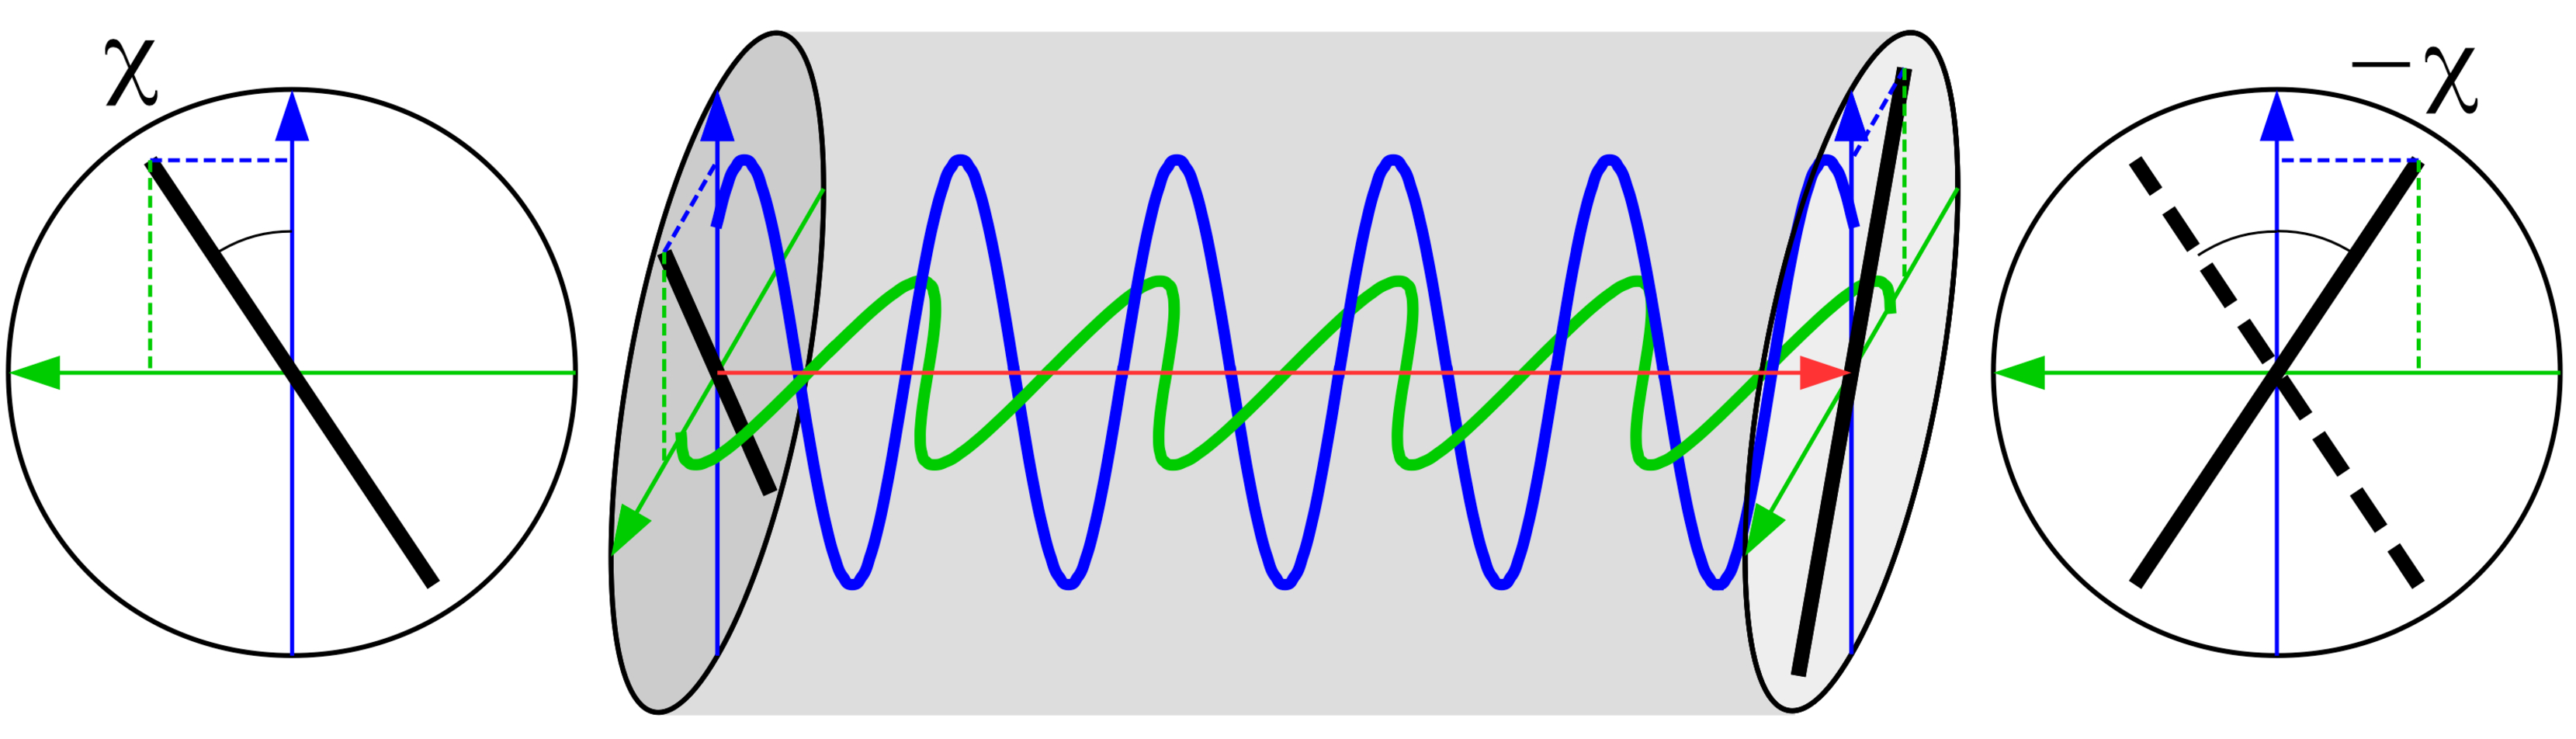
\includegraphics[width=1.0\textwidth]{simons_observatory/hwp_satoru.pdf}
    \caption{HWPを通過することで偏光角が変化することを示した概念図~\cite{takakura_PhD}。
    左から右に向かって直線偏光がHWPを通過している。}
    \label{fig:so-hwp_satoru}
\end{figure}

\section{偏光角較正の重要性とその手法}
\subsection{偏光角の誤較正に伴う偏光の漏れ込み}
CMB偏光観測実験でのBモード観測において、検出器の偏光角$\theta_{\mathrm{det}}$を精度よく知ることは極めて重要である。
その重要性を示すため、本項では偏光角の誤較正が観測されたBモード偏光にどのような影響を及ぼすかを考え、
SOにおいての要求偏光角較正精度を定める。

今、すべての検出器における偏光角を $\delta \theta$ だけ誤って較正してしまったとすると、
観測されるストークスパラメータ $Q_{\mathrm{obs}},\ U_{\mathrm{obs}}$ は真のストークスパラメータ $Q,\ U$ に対して
\begin{align}
    Q_{\mathrm{obs}} \pm iU_{\mathrm{obs}} &= e^{\pm i2\delta\theta}\qty(Q \pm iU) \\
    &= e^{\pm i2\delta\theta}\sum_{\ell=2}^{\infty}\sum_{m=-\ell}^{\ell} {}_{\pm 2}a_{\ell m}\ {}_{\pm 2}Y_{\ell m}(\theta, \phi)
\end{align}
とバイアスされた値となる\cite{so:Keating_2013}\cite{so:Kaufman_2014}。
Eモード、Bモード偏光を表現する係数 $a_{\ell m}^{E}, a_{\ell m}^{B}$ を用いると、
スピン2の球面調和関数で展開する際の係数 ${}_{\pm 2}a_{\ell m}$ は
\begin{equation}
    {}_{\pm 2}a_{\ell m} = -\qty(a_{\ell m}^{E} \pm i a_{\ell m}^{B})
\end{equation}
であるから
\begin{align}
    Q_{\mathrm{obs}} \pm iU_{\mathrm{obs}} &= \sum_{\ell=2}^{\infty}\sum_{m=-\ell}^{\ell} \qty[-\qty(a_{\ell m}^{E} \pm i a_{\ell m}^{B})]e^{\pm i2\delta\theta}\ {}_{\pm 2}Y_{\ell m}(\theta, \phi) \\
    &= \sum_{\ell=2}^{\infty}\sum_{m=-\ell}^{\ell} \qty[-\qty(a_{\ell m,\,\mathrm{obs}}^{E} \pm i a_{\ell m,\,\mathrm{obs}}^{B})] {}_{\pm2}Y_{\ell m}(\theta, \phi)
\end{align}
が観測されることとなる。したがって、パワースペクトル
\begin{equation}
    C_{\ell}^{XX'} = \dfrac{1}{2\ell+1}\sum_{m=-\ell}^{l}\left\langle \qty(a_{\ell m}^{X})^{*} a_{\ell m}^{X'} \right\rangle
\end{equation}
は、偏光角の誤較正によって
\begin{equation}
    \label{eq:so-leakage}
    \mqty( C_{\mathrm{obs},\,\ell}^{TT} \\[1ex]
           C_{\mathrm{obs},\,\ell}^{TE} \\[1ex]
           C_{\mathrm{obs},\,\ell}^{TB} \\[1ex]
           C_{\mathrm{obs},\,\ell}^{EE} \\[1ex]
           C_{\mathrm{obs},\,\ell}^{BB} \\[1ex]
           C_{\mathrm{obs},\,\ell}^{EB} )
    = \mqty( 1 & 0 & 0 & 0 & 0 & 0 \\[1ex]
             0 & \cos\qty(2\delta\theta) & 0 & -\sin\qty(2\delta\theta) & 0 & 0 \\[1ex]
             0 & \sin\qty(2\delta\theta) & 0 & \cos\qty(2\delta\theta) & 0 & 0 \\[1ex]
             0 & 0 & 0 & \cos^2\qty(2\delta\theta) & \sin^2\qty(2\delta\theta) & -\sin\qty(4\delta\theta) \\[1ex]
             0 & 0 & 0 & \sin^2\qty(2\delta\theta) & \cos^2\qty(2\delta\theta) & \sin(4\delta\theta) \\[1ex]
             0 & 0 & 0 & \sin\qty(4\delta\theta)/2 & -\sin\qty(4\delta\theta)/2 & \cos\qty(4\delta\theta)/2 )
    \mqty( C_{\ell}^{TT} \\[1ex]
              C_{\ell}^{TE} \\[1ex]
              C_{\ell}^{TB} \\[1ex]
              C_{\ell}^{EE} \\[1ex]
              C_{\ell}^{BB} \\[1ex]
              C_{\ell}^{EB} )
\end{equation}
となる。
標準宇宙モデルが正しく、原始密度ゆらぎがパリティ不変だった場合では $C_{\ell}^{TB}=C_{\ell}^{EB}=0$ であるが、
それでも偏光角の誤較正は $C_{\ell}^{EE}$ から $C_{\ell}^{BB}$ への漏れ込みを引き起こす。式\eqref{eq:so-leakage}から算出すると
\begin{equation}
    \label{eq:so-EtoBleakage}
    C_{\mathrm{obs},\,\ell}^{BB} = \sin^2\qty(2\delta\theta)C_{\ell}^{EE} + \cos^2\qty(2\delta\theta)C_{\ell}^{BB}
\end{equation}

式\eqref{eq:so-EtoBleakage}に基づき、偏光角の誤較正が $C_{\ell}^{EE}$ から 
$C_{\mathrm{obs}, \ell}^{BB}$ への漏れ込みとして及ぼす影響を図\ref{fig:so-EtoBleakage}に示す\footnote{図の作成には\href{http://class-code.net}{CLASS}を用いた。}。
テンソルスカラー比$r$は、BICEP2/KeckとPlanckの統合解析によって得られた$r=0.032$を上限とし、$r=0.001$までを描いた。
誤較正の目安として、 $\delta\theta = 10\tcdegree, 1\tcdegree, 0.1\tcdegree$ の場合をプロットした。
$\delta\theta=10\tcdegree$や$\delta\theta=1\tcdegree$では$C_{\ell}^{EE}$の漏れ込みが$C_{\ell}^{BB}$の大きさ以上に残ってしまう。
この図からは、偏光角較正の要求精度が$\delta\theta < 0.1\tcdegree$であることが直感的に理解できる。

偏光角較正の要求精度は望遠鏡の感度や、ノイズなどにも依存する。
SOでは、ノイズとして最も悲観的な場合を考えた場合でも
$\delta\theta \leq 0.1\tcdegree$であればこの漏れ込みが生むテンソルスカラー比$r$への系統誤差は無視できるほどに小さくなる~\cite{so:Bryan_2018}。
以上の理由から、SOでの偏光角較正の要求精度を $\delta\theta \leq 0.1\tcdegree$ と定める。

\begin{figure}[H]
    \centering
    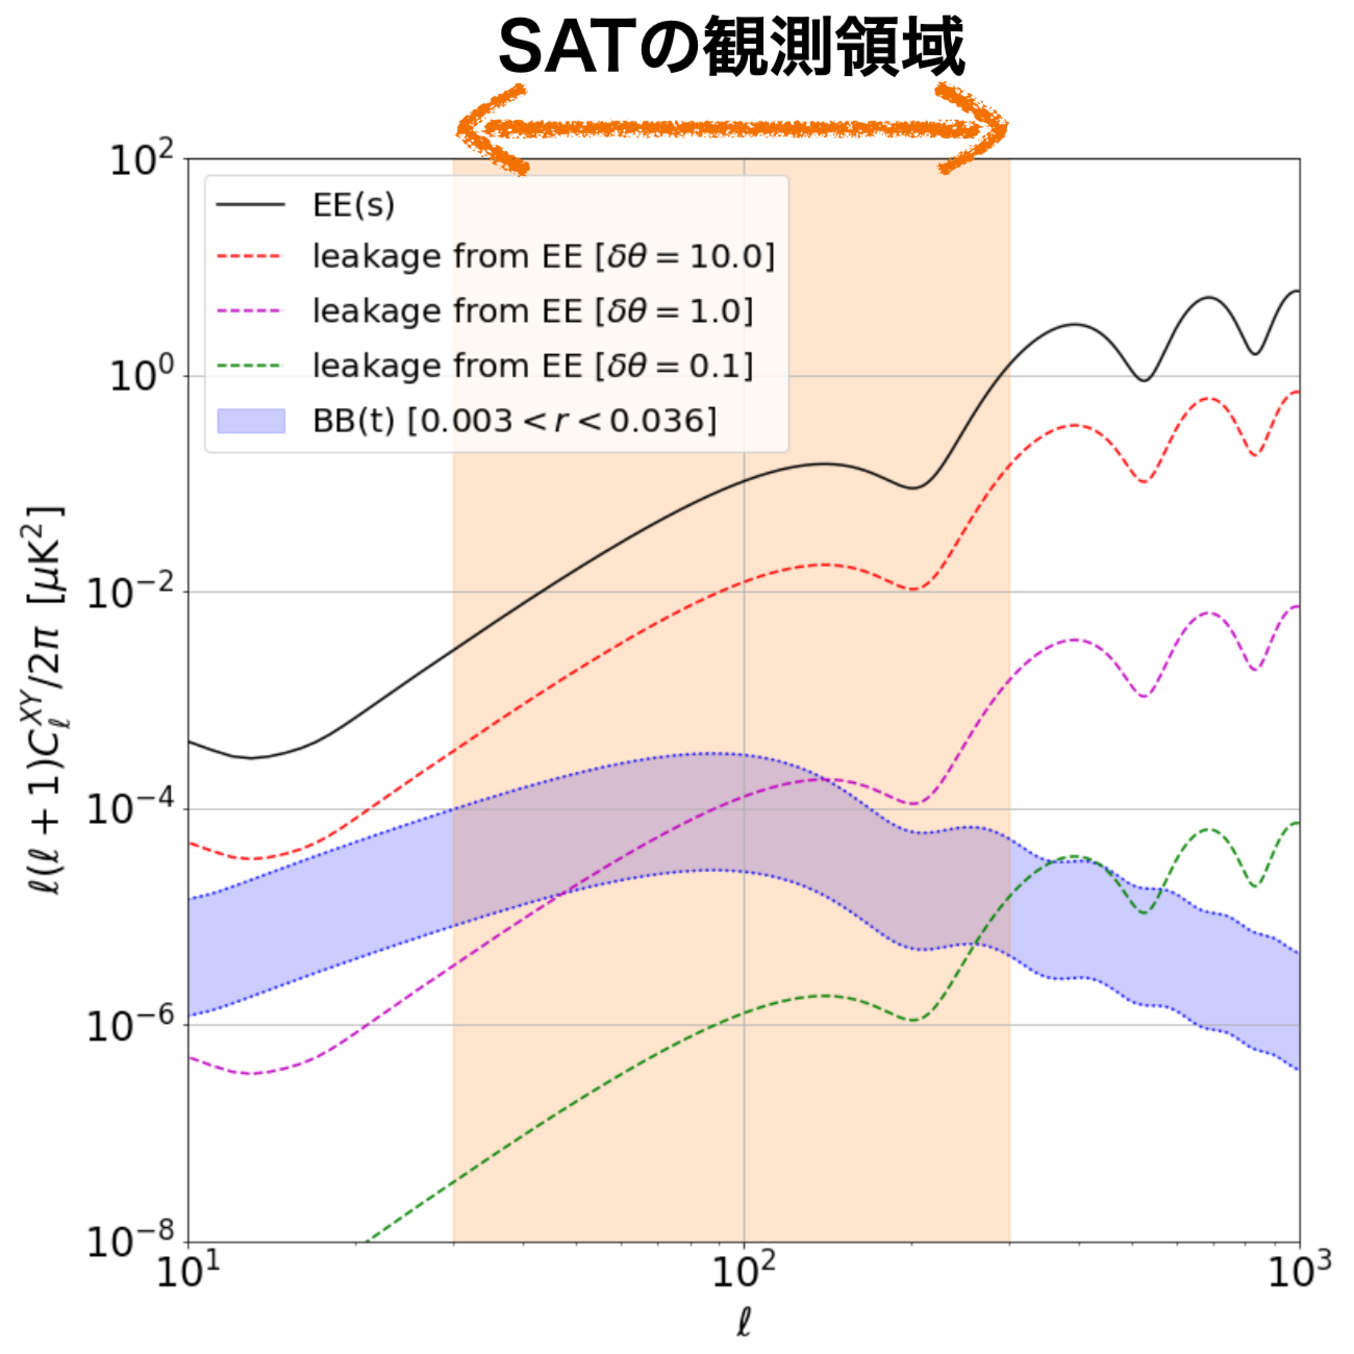
\includegraphics[width=0.80\textwidth]{simons_observatory/EtoB_leakage.pdf}
    \caption{偏光角の誤較正が $C_{\ell}^{EE}$ から $C_{\ell}^{BB}$ への漏れ込みとして及ぼす影響。
    BICEP/KeckとPlanckの統合解析によって得られた$r=0.032$を上限とし、$r=0.001$までを描いた。}
    \label{fig:so-EtoBleakage}
\end{figure}

\subsection{偏光角較正手法}
偏光角較正には、検出器間の相対的な偏光角を較正する相対角度較正と、
天球面上においてどの向きに検出器の偏光角が対応するかを較正する絶対角度較正が存在する。
本項では代表的な較正手法を紹介したのち、先行研究においてどのような手法をとり、その精度がどの程度であったかをまとめる。
\subsubsection{牡牛座かに星雲 (Tau A)}
Tau Aは北天に昇る、強い直線偏光を放射する超新星残骸である。
その光の偏光角は観測周波数に依存している可能性が指摘されており、さらに高分解能望遠鏡による観測では
天体表面上の異なる位置での偏光方向の違いが見えるため、偏光角を一意に決定することが難しく、
系統誤差の見積もりに$0.4\tcdegree$の不定性があるという課題がある。
また、偏光角は他の実験の観測結果にも依存しており、これらが潜在的な系統誤差として存在する。
小さい天体であるために検出器全てを一度に照らすことができず、
全ての検出器を較正するためにはスキャンを行う必要があるため、
全検出器を同時に構成することができない。
さらに、SOの拠点であるチリのアタカマ砂漠は南半球に位置しており、TauA の昇る高度が高くないためSATでは検出器の一部でしか観測できない。
\subsubsection{ケンタウルス座A (Cen A)}
Cen Aは南天に昇る、直線偏光を放射する電波銀河である。
QUaD実験にて、$0.5\tcdegree$の絶対角度較正精度が保証された検出器群を用いて\SI{90}{GHz}と\SI{150}{GHZ}の波長帯で観測され、その偏光角が測定されている~\cite{so:Zemcov_2010}。
南天に登るため南半球で比較的観測しやすいが、偏光角の観測周波数依存性や高分解能望遠鏡で見える内部構造の影響、他の実験の観測結果による依存といったTau Aと同様の要因による系統誤差を持ち得る。
\subsubsection{月}
月はその表面で反射された光が月の中心から放射状に広がった偏光信号となる。
月の観測は TauA と同様に観測する月の表面上の位置による偏光角の違いが問題となり、ポインティング精度由来の系統誤差を生じる。
また、月は非常に明るいためTES検出器のダイナミックレンジを超えてしまい、SATでは観測が困難である。
\subsubsection{誘電体シート}
誘電体シートとは、膜状に張られたポリマーによって環境熱放射を反射させ、直線偏光を作り出す装置である。
その厚みを変えることで明るさの調整が容易であるが、望遠鏡の視野をすべて覆うためには装置が大型化する傾向にある。
また、周波数ごとに偏光特性が異なるため、較正に使用するためには高精度な周波数依存性の測定が必要である。

\subsubsection{デンスワイヤーグリッド}
デンスワイヤーグリッドは、金属ワイヤーを入射光に対して十分短い間隔で平行に張り巡らせた光学素子である。
近似的にはワイヤーが張られた方向に対しては電流を流すが、それに直行する方向には電流を流さない金属板として振る舞う。
そのため、入射光がワイヤーに沿った方向に偏光している場合には反射され、直行する方向に偏光している光は透過する。

デンスワイヤーグリッドは口径に対して平行に設置してしまうと検出器アレイとの間に多重反射が生じ、系統誤差を生じる。
これを抑制するため、デンスワイヤーグリッドを口径に対して傾けて設置する使用例が多い。
望遠鏡の口径を覆い、全検出器を同時に較正するためにはデンスワイヤーグリッド自体が大型化する必要があり、
作成する際にはワイヤー間隔を高精度に制御、長期間保つことが困難である。

\subsubsection{スパースワイヤーグリッド}
スパースワイヤーグリッドは、金属ワイヤーを入射光に対して十分長い間隔で平行に張り巡らせた光学素子である。
原理は\ref{sec:wiregrid_principle}節にて後述するが、環境熱放射をワイヤーが反射することによりワイヤーに沿った方向に偏光した光を作り出す。

スパースワイヤーグリッドはワイヤー間隔が広いために多重反射を起こしにくく、望遠鏡の口径に対して平行に設置することができる。
そのため、デンスワイヤーグリッドよりも小型化が可能であり、製造難易度が比較的低い。
また、ワイヤー間隔が十分長いとみなせる範囲においては周波数依存性が小さいため、
広い周波数帯で均一に偏光を生成することが可能である。

\subsubsection{自己較正}
標準宇宙モデルでは $C_{\ell}^{EB}=0$ である。
これを利用して、相対角度較正を十分に行なった上で $C_{\ell}^{EB} = 0$ とおくことで
$\delta\theta$ を求め、絶対角度較正を行う手法を自己較正と呼ぶ。
自己較正の精度は相対角度較正の精度と検出データ量に依存するため、検出器数が増大によって精度の向上が期待される。
しかし、$C_{\ell}^{EB}=0$ を仮定してしまうため、標準宇宙モデルを超えるような物理に対する感度を捨てる可能性がある。
別の言い方をすれば、標準宇宙モデルを仮定したデータ解析となってしまう。そのため、この自己較正以外の手法を用いて絶対角度較正を行うことが重要である。

\subsubsection{偏光角較正手法のまとめとスパースワイヤーグリッドの採用理由}
先行研究における偏光角較正の手法と、その精度を表\ref{tab:so-polarization_calibration}にまとめる。
いずれの手法においても、精度 $\delta\theta < 0.1\tcdegree$ を達成したものはない。
SATではスパースワイヤーグリッドを用いた偏光角較正を採用することで、この精度を目指す。
スパースワイヤーグリッドは周波数依存性が小さく、広い周波数帯で均一に直線偏光を作り出せるという点と、
望遠鏡の視野を全て覆うような装置として作成可能なため、全ての検出器を同時に較正可能である点が優れている。
また、自己較正のように標準宇宙モデルを超える物理に対する感度を捨てることもない。
このような理由から、他の手法よりも系統誤差の削減が期待でき、採用に至った。
\begin{table}[H]
    \centering
    \caption[先行研究における偏光角較正手法とその精度の比較]{先行研究における偏光角較正手法とその絶対角度較正精度の比較。
    どの手法においても$\delta\theta < 0.1\tcdegree$を達成したものはない。}
    \begin{tabular}{cccc}
        \hline
        実験 & 観測周波数帯 [GHz] & 較正手法 & $\delta\theta$ \\
        \hline
        \hline
        \multirow{2}{*}{POLARBEAR\cite{so:polarbear_cal}} & \multirow{2}{*}{$150$} & Tau A & $0.43\tcdegree$ \\
                                                          &                        & 自己較正\footnotemark[1] & $0.2\tcdegree$ \\
        \hline
        DASI\cite{so:Leitch_2002} & $26\sim36$ & 月, デンスワイヤーグリッド & $0.4\tcdegree$ \\
        \hline
        BICEP\cite{so:Takahashi_2008} & $100,\,150,\,220$ & 誘電体シート & $0.7\tcdegree$ \\
        \hline
        BICEP2\cite{so:bicep2_syserr} & $150$ & 自己較正\footnotemark[1] & $1\tcdegree$\\
        \hline
        % BICEP3\cite{so:bicep3} & $95$ & デンスワイヤーグリッド & $0.3\tcdegree$ \\
        \multirow{2}{*}{SPTpol\cite{so:Hanson_2013}} & $150$ & \multirow{2}{*}{デンスワイヤーグリッド} & $1\tcdegree$ \\
                                                     & $95$  & & $1.5\tcdegree$ \\
        \hline
        \multirow{3}{*}{ABS\cite{so:Kusaka_2018}} & \multirow{3}{*}{$145$} & スパースワイヤーグリッド & $1.1\tcdegree$ \\
                                                  &                        & Tau A & $1.9\tcdegree$ \\
                                                  &                        & 自己較正\footnotemark[1] & $1.6\tcdegree$ \\
        \hline
        \multirow{2}{*}{QUIET\cite{so:Bischoff_2011}} & \multirow{2}{*}{$43,\,94$} & 月 & $1\tcdegree$ \\
                                                      &                            & Tau A, スパースワイヤーグリッド & $3\tcdegree$ \\
        \hline
        \multirow{3}{*}{SPT-3G\cite{so:SPT3G}} & $90$  & \multirow{3}{*}{Cen A} & $2.0\tcdegree$ \\
                                               & $150$ &                        & $2.2\tcdegree$ \\
                                               & $220$ &                        & $4.5\tcdegree$ \\
        \hline
    \end{tabular}
    \label{tab:so-polarization_calibration}
\end{table}
\footnotetext[1]{標準宇宙モデル$(C_{\ell}^{EB}=0)$を仮定した手法であり、究極の較正手段とはなり得ない。}
\end{document}